% HealthStack project README, LaTeX version of docs/README.md (same content).
% Compile from the docs/ folder so the ER image path resolves:
%   pdflatex README.tex   (run twice for the table of contents)
\documentclass[11pt,a4paper]{article}

\usepackage[T1]{fontenc}
\usepackage[utf8]{inputenc}
\usepackage[margin=2cm]{geometry}
\usepackage{lmodern}
\usepackage{amsmath,amssymb}
\usepackage{graphicx}
\usepackage{booktabs}
\usepackage{tabularx}
\usepackage{array}
\usepackage{enumitem}
\usepackage{xcolor}
\usepackage{listings}
\usepackage[hidelinks]{hyperref}

\setlist{itemsep=2pt,topsep=4pt}
\setlength{\parskip}{4pt}
\setlength{\parindent}{0pt}
\renewcommand{\arraystretch}{1.25}
\newcolumntype{L}{>{\raggedright\arraybackslash}X}
\newcommand{\code}[1]{\texttt{#1}}
\newcommand{\fk}{$\rightarrow$\,}

\definecolor{codebg}{RGB}{246,247,249}
\definecolor{codekw}{RGB}{0,92,158}
\definecolor{codecm}{RGB}{110,120,130}
\lstset{
  basicstyle=\ttfamily\footnotesize,
  backgroundcolor=\color{codebg},
  keywordstyle=\color{codekw}\bfseries,
  commentstyle=\color{codecm}\itshape,
  breaklines=true,
  breakatwhitespace=false,
  columns=fullflexible,
  keepspaces=true,
  frame=single,
  rulecolor=\color{codebg},
  xleftmargin=4pt,
  xrightmargin=4pt,
  aboveskip=6pt,
  belowskip=6pt
}
\lstdefinestyle{sql}{language=SQL, morekeywords={START,TRANSACTION,COMMIT,ROLLBACK,UPDATE,FOR,DATE_ADD,UTC_TIMESTAMP,INTERVAL,DAY,TRUE,NULL,JOIN,ON,DESC}}
\lstdefinestyle{bash}{language=bash, morecomment=[l]{--}}

\title{\textbf{HealthStack}}
\author{}
\date{}

\begin{document}
\maketitle
\vspace{-3em}

HealthStack is a hospital management system built on a MySQL database. It covers the part of a hospital's day that a patient actually sees: finding a doctor, booking a slot, the consultation, the prescription and the bill.

There are three kinds of users, and each gets their own screens:

\begin{itemize}
  \item \textbf{Patients} register and log in, browse departments and doctors, see a doctor's free slots, and book, cancel or reschedule appointments. They can see their past visits with the prescription and bill for each one.
  \item \textbf{Doctors} see today's queue. Opening an appointment shows the patient's details and their full visit history. Completing a visit records the prescription, and the system creates the bill.
  \item \textbf{Pharmacists} see every unpaid bill with the medicines prescribed, and mark bills as paid.
\end{itemize}

The database does more than store rows. Constraints and triggers enforce the hospital's rules, such as no double-booking, no prescription for a cancelled visit, and no change to a bill once it is issued. They apply no matter which program writes the data. Every multi-step action runs as a transaction, so it either completes fully or leaves nothing behind.

\begin{center}
\small
\begin{tabularx}{\textwidth}{l L L}
\toprule
\textbf{Layer} & \textbf{Technology} & \textbf{Folder} \\
\midrule
Database & MySQL 8.0.16+ (tables, constraints, triggers) & \code{backend/schema}, \code{backend/seed}, \code{backend/triggers} \\
Backend  & Python, FastAPI, \code{mysql-connector-python} & \code{backend/} \\
Frontend & React, Vite, Tailwind CSS & \code{frontend/} \\
\bottomrule
\end{tabularx}
\end{center}

\tableofcontents

% ---------------------------------------------------------------------------
\section{Running the project}

\begin{lstlisting}[style=bash]
# 1. Database (from the project root, inside the mysql client)
mysql -u root -p
mysql> SOURCE backend/schema/table.sql;   -- all tables + all triggers (wipes existing data)
mysql> SOURCE backend/seed/seed.sql;      -- demo data

# 2. Backend (http://127.0.0.1:8000, API docs at /docs)
cd backend
cp .env.example .env                      # then fill in your MySQL user and password
pip install -r requirements.txt
python server.py

# 3. Frontend (http://localhost:5173)
cd frontend
npm install
npm run dev
\end{lstlisting}

Demo logins (password \code{demo123} for all): \code{patient@demo.com}, \code{doctor@demo.com}, \code{pharmacist@demo.com}.

% ---------------------------------------------------------------------------
\section{ER model}

\begin{center}
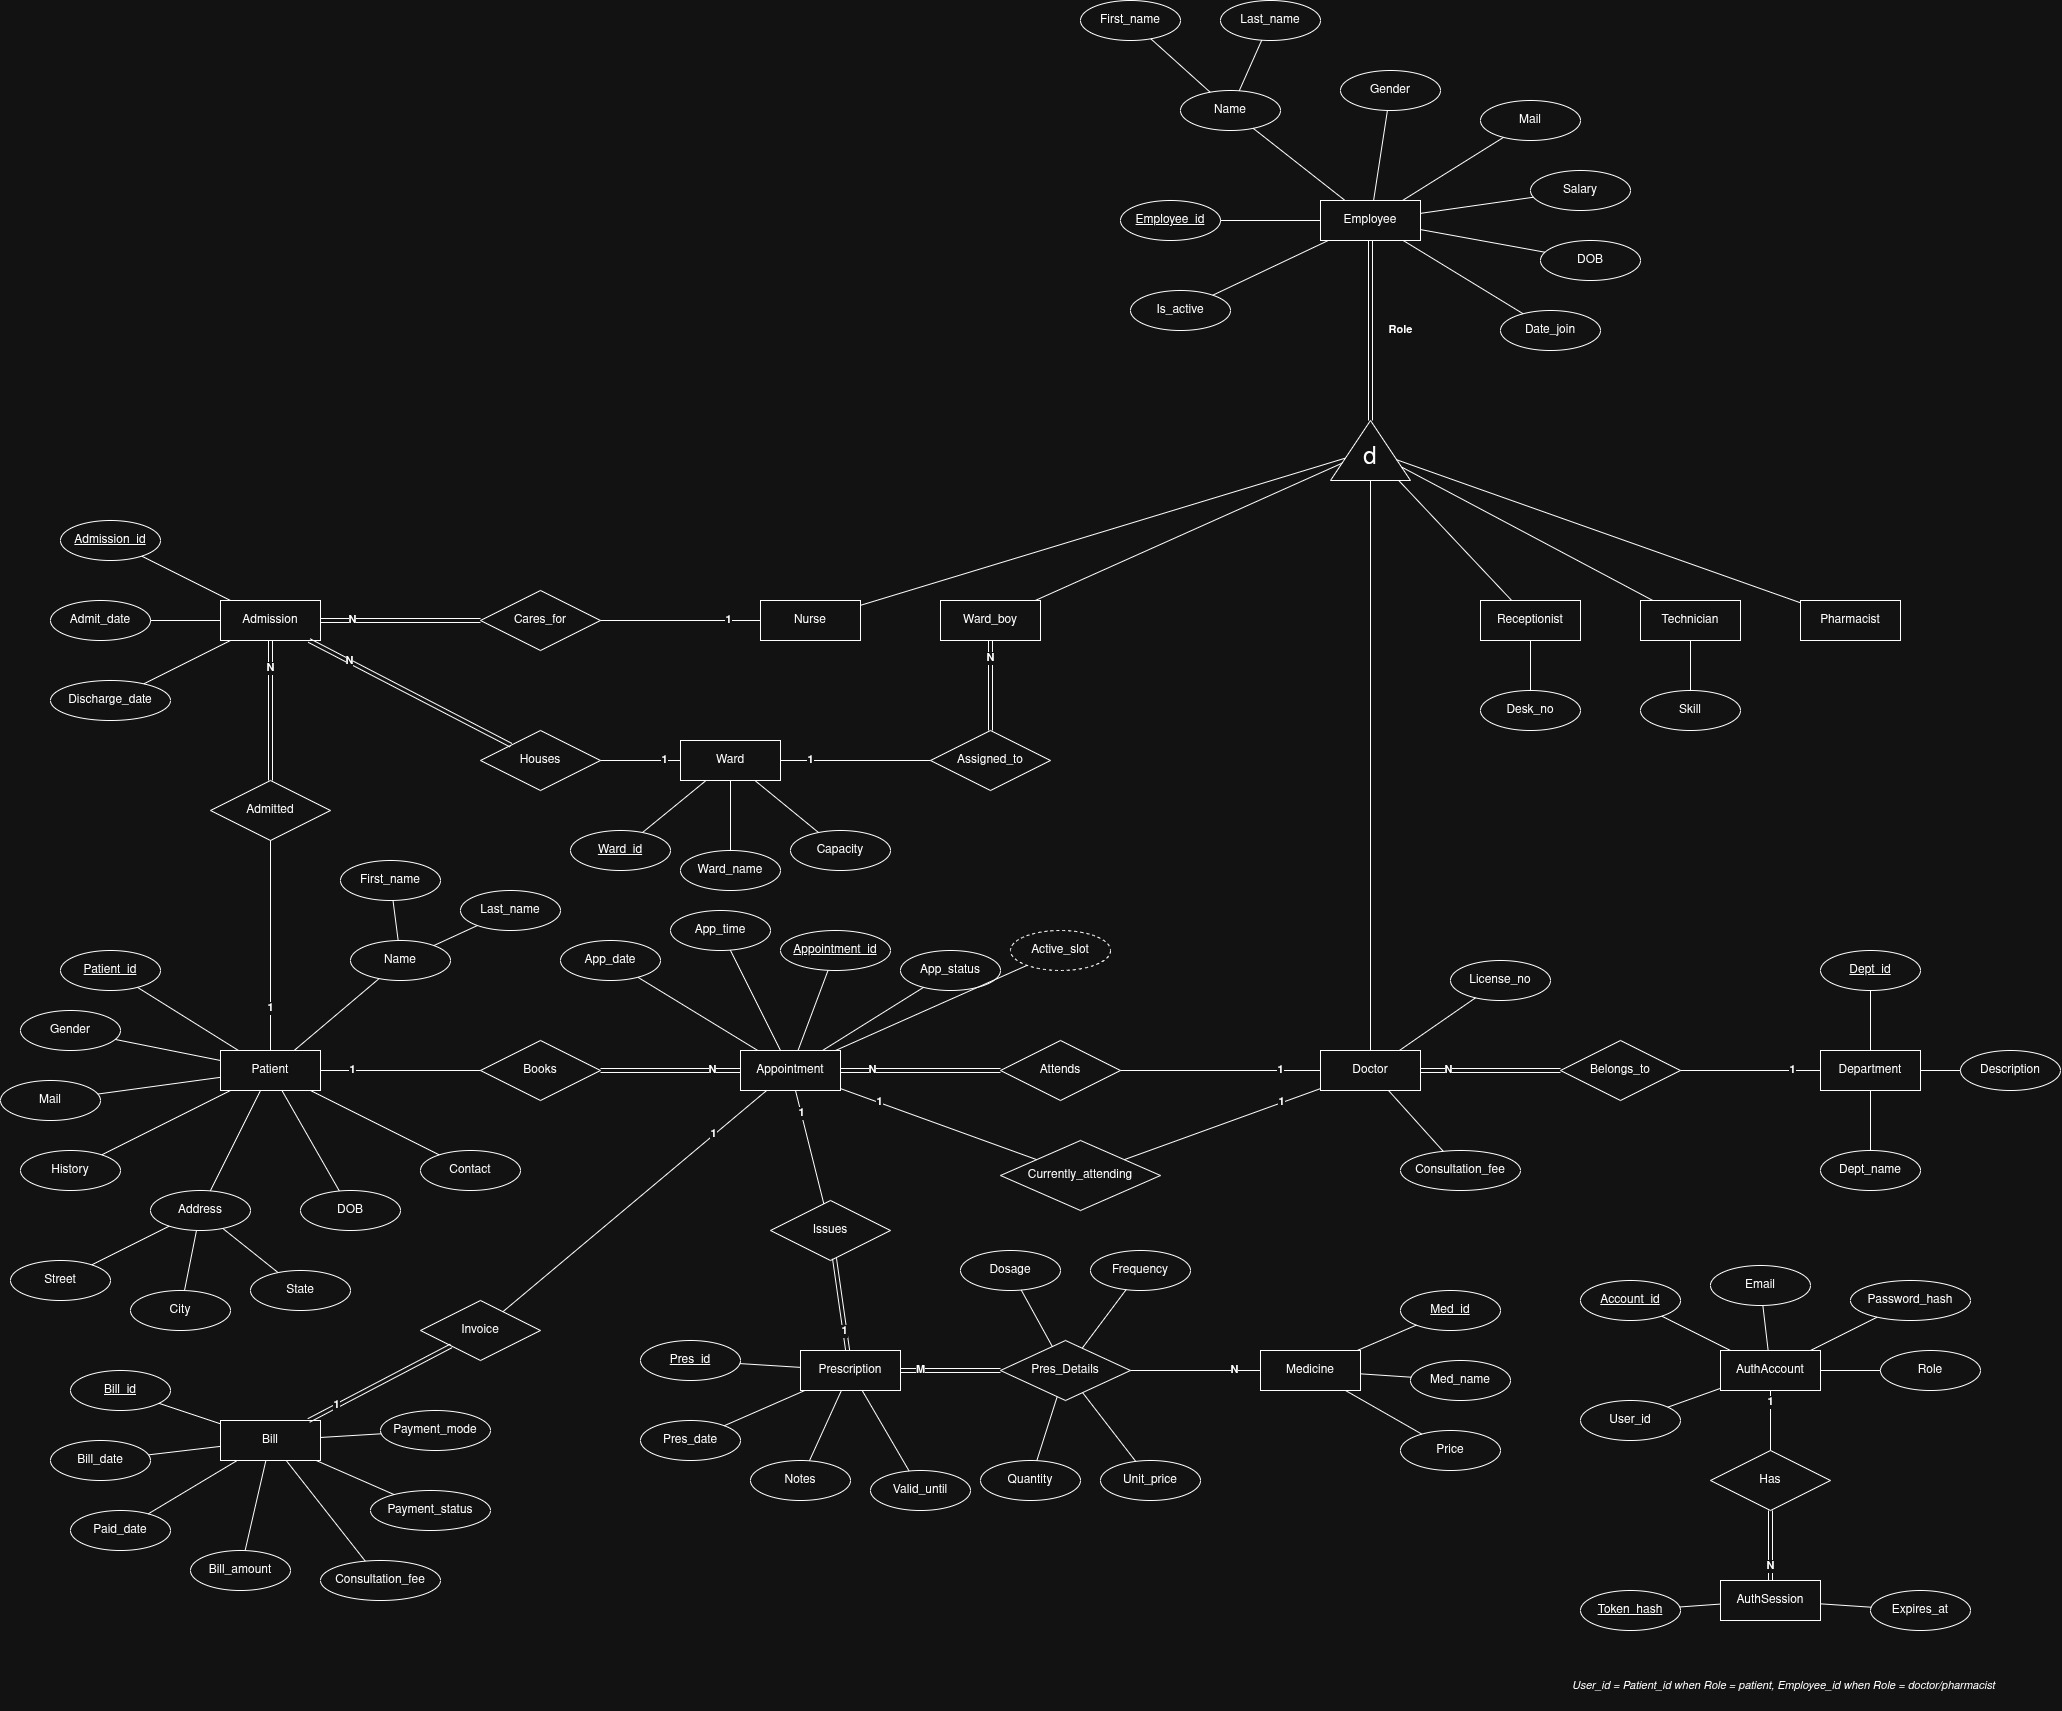
\includegraphics[width=\textwidth]{diagrams/HealthStack_ER_updated.jpg}
\end{center}

\begin{itemize}
  \item \textbf{Employee} is specialised into Doctor, Nurse, Ward\_boy, Receptionist, Technician and Pharmacist. The specialisation is \textbf{disjoint} (\code{d}), \textbf{total} (double line), and decided by the attribute \code{Role}.
  \item \code{Name} and \code{Address} are composite attributes; \code{Active\_slot} is a derived attribute (dashed).
  \item \code{Pres\_Details} is an M:N relationship with its own attributes (\code{Dosage}, \code{Quantity}, \code{Frequency}, \code{Unit\_price}).
  \item \code{AuthAccount.User\_id} is a \code{Patient\_id} when \code{Role} = patient, and an \code{Employee\_id} otherwise (note at the bottom of the diagram).
  \item \textbf{Technician}, \textbf{Admission} and their relationships (Admitted, Houses, Cares\_for) are planned scope. They are in the diagram but not yet in \code{table.sql}.
\end{itemize}

% ---------------------------------------------------------------------------
\section{Schema and normal forms}

All tables are created by \code{backend/schema/table.sql}. \textbf{Bold} marks the primary key, \fk marks a foreign key, and (U) marks a \code{UNIQUE NOT NULL} column.

\begin{center}
\small
\begin{tabularx}{\textwidth}{l L}
\toprule
\textbf{Table} & \textbf{Columns} \\
\midrule
\code{Department}   & \textbf{Dept\_id}, Dept\_name (U), Description \\
\code{Employee}     & \textbf{Employee\_id}, First\_name, Last\_name, Gender, DOB, Date\_join, Mail (U), Salary, Role, Is\_active \\
\code{Doctor}       & \textbf{Employee\_id} \fk Employee, License\_no (U), Current\_appointment\_id, Dept\_id \fk Department, Consultation\_fee \\
\code{Nurse}        & \textbf{Employee\_id} \fk Employee \\
\code{Ward}         & \textbf{Ward\_id}, Ward\_name (U), Capacity \\
\code{Ward\_boy}    & \textbf{Employee\_id} \fk Employee, Ward\_id \fk Ward \\
\code{Receptionist} & \textbf{Employee\_id} \fk Employee, Desk\_no \\
\code{Pharmacist}   & \textbf{Employee\_id} \fk Employee \\
\code{Patient}      & \textbf{Patient\_id}, First\_name, Last\_name, Gender, DOB, Mail, Contact, Street, City, State, History \\
\code{Appointment}  & \textbf{Appointment\_id}, Patient\_id \fk Patient, Doctor\_id \fk Doctor, App\_date, App\_time, App\_status, Active\_slot (generated) \\
\code{Prescription} & \textbf{Pres\_id}, Appointment\_id \fk Appointment (U), Pres\_date, Notes, Valid\_until \\
\code{Medicine}     & \textbf{Med\_id}, Med\_name, Price \\
\code{Pres\_Details} & \textbf{(Pres\_id \fk Prescription, Med\_id \fk Medicine)}, Dosage, Quantity, Frequency, Unit\_price \\
\code{Bill}         & \textbf{Bill\_id}, Appointment\_id \fk Appointment (U), Consultation\_fee, Bill\_amount, Bill\_date, Paid\_date, Payment\_status, Payment\_mode \\
\code{AuthAccount}  & \textbf{Account\_id}, Email (U), Password\_hash, Role, User\_id; \code{UNIQUE (Role, User\_id)} \\
\code{AuthSession}  & \textbf{Token\_hash}, Account\_id \fk AuthAccount, Expires\_at \\
\bottomrule
\end{tabularx}
\end{center}

ER to tables: composite attributes are split into columns, each subclass is a table whose primary key is also a foreign key to \code{Employee}, and 1:1 relationships are a \code{UNIQUE} foreign key. \code{CHECK} constraints cover values such as gender, status, \code{Salary >= 0} and \code{Date\_join > DOB}.

\code{Active\_slot} is \code{1} for a live appointment and \code{NULL} for a cancelled one. \code{UNIQUE (Doctor\_id, App\_date, App\_time, Active\_slot)} and the same index on \code{Patient\_id} stop double-booking. A unique index allows repeated \code{NULL}s, so a cancelled slot can be booked again.

\subsection{Normal forms used}

\begin{itemize}
  \item \textbf{1NF}: every value is atomic, and the table has a key.
  \item \textbf{2NF}: 1NF, and no non-prime attribute depends on only part of a candidate key.
  \item \textbf{3NF}: for every non-trivial FD $X \rightarrow A$, $X$ is a superkey or $A$ is prime (no transitive dependency).
  \item \textbf{BCNF}: for every non-trivial FD $X \rightarrow A$, $X$ is a superkey.
\end{itemize}

A table whose candidate keys are all single attributes is automatically in 2NF.

\subsection{Normal form of each table}

\begin{center}
\footnotesize
\begin{tabularx}{\textwidth}{>{\raggedright\arraybackslash}p{2.1cm} >{\raggedright\arraybackslash}p{2.9cm} >{\raggedright\arraybackslash}p{3.3cm} l L}
\toprule
\textbf{Table} & \textbf{Candidate keys} & \textbf{Non-trivial FDs} & \textbf{Highest NF} & \textbf{Reason} \\
\midrule
\code{Department}   & Dept\_id; Dept\_name & each key $\rightarrow$ all & BCNF & Only keys determine anything \\
\code{Employee}     & Employee\_id; Mail & each key $\rightarrow$ all & BCNF & Role $\nrightarrow$ Salary (doctors 101 and 102 earn different salaries) \\
\code{Doctor}       & Employee\_id; License\_no & each key $\rightarrow$ all & BCNF & Dept\_id $\nrightarrow$ Consultation\_fee: the fee is per doctor \\
\code{Nurse}        & Employee\_id & none & BCNF & Single column \\
\code{Ward}         & Ward\_id; Ward\_name & each key $\rightarrow$ all & BCNF & Only keys determine anything \\
\code{Ward\_boy}    & Employee\_id & Employee\_id $\rightarrow$ Ward\_id & BCNF & A ward has many ward boys, so Ward\_id is not a key \\
\code{Receptionist} & Employee\_id & Employee\_id $\rightarrow$ Desk\_no & BCNF & Desks can be shared \\
\code{Pharmacist}   & Employee\_id & none & BCNF & Single column \\
\code{Patient}      & Patient\_id & Patient\_id $\rightarrow$ all & BCNF & Mail is nullable and not unique; City $\nrightarrow$ State (city names repeat across states) \\
\code{Appointment}  & Appointment\_id & key $\rightarrow$ all; \textbf{App\_status $\rightarrow$ Active\_slot} & \textbf{2NF} & See note 1 \\
\code{Prescription} & Pres\_id; Appointment\_id & each key $\rightarrow$ all & BCNF & One prescription per appointment \\
\code{Medicine}     & Med\_id & Med\_id $\rightarrow$ all & BCNF & Med\_name is not unique \\
\code{Pres\_Details} & (Pres\_id, Med\_id) & (Pres\_id, Med\_id) $\rightarrow$ rest & BCNF & See note 2 \\
\code{Bill}         & Bill\_id; Appointment\_id & each key $\rightarrow$ all; \textbf{$\emptyset \rightarrow$ Consultation\_fee} & \textbf{2NF} & See note 3 \\
\code{AuthAccount}  & Account\_id; Email; (Role, User\_id) & each key $\rightarrow$ all & BCNF & Neither Role nor User\_id alone determines anything (no partial dependency) \\
\code{AuthSession}  & Token\_hash & Token\_hash $\rightarrow$ all & BCNF & An account can have many sessions \\
\bottomrule
\end{tabularx}
\end{center}

\textbf{14 of 16 tables are in BCNF.} The two exceptions are deliberate or easy to fix:

\begin{enumerate}
  \item \textbf{Appointment} stores the derived column \code{Active\_slot}, so $\text{Appointment\_id} \rightarrow \text{App\_status} \rightarrow \text{Active\_slot}$ is transitive. MySQL computes the column itself (\code{GENERATED ... STORED}), so it can never disagree with \code{App\_status}. It exists only to make the unique index skip cancelled rows, which MySQL can't do any other way. Without it, the table is in BCNF.
  \item \textbf{Pres\_Details} might look like it has the partial dependency $\text{Med\_id} \rightarrow \text{Unit\_price}$. It doesn't: \code{Unit\_price} is the price at the time of prescribing, copied by a trigger, so the same medicine can have different prices in older and newer prescriptions. Dosage and quantity also vary per pair (medicine 1 is 10 tablets in prescription 1 and 6 in prescription 6).
  \item \textbf{Bill}: trigger \code{trg\_bill\_bi} always sets \code{Consultation\_fee = 200}, so the column is a constant. Any non-key attribute then determines it (for example $\text{Bill\_date} \rightarrow \text{Consultation\_fee}$), which breaks 3NF. Copying the doctor's own \code{Consultation\_fee} into the bill makes the table BCNF.
\end{enumerate}

% ---------------------------------------------------------------------------
\section{Triggers}

\code{table.sql} installs all 25 triggers and one stored procedure. The same code is split by topic in \code{backend/triggers/} (\code{install.sql} reinstalls them without touching data). Each rejects bad data with \code{SIGNAL SQLSTATE '45000'}, which the API returns as an HTTP 409.

\begin{center}
\footnotesize
\begin{tabularx}{\textwidth}{>{\raggedright\arraybackslash}p{4.6cm} >{\raggedright\arraybackslash}p{3.6cm} L}
\toprule
\textbf{Trigger(s)} & \textbf{Table (event)} & \textbf{Rule} \\
\midrule
\code{check\_employee\_role} (procedure) & -- & Fails unless the employee exists with the given \code{Role} \\
\code{trg\_<subclass>\_role\_bi / \_bu} (10) & 5 subclass tables (insert, update) & Row allowed only if \code{Employee.Role} matches the table: the \textbf{disjoint} specialisation \\
\code{trg\_employee\_role\_lock} & Employee (update) & \code{Role} can't change while the employee has a subclass row \\
\code{trg\_employee\_dates\_bi / \_bu} & Employee (insert, update) & DOB in the past, join date not in the future, at least 18 when joining \\
\code{trg\_patient\_dob\_bi / \_bu} & Patient (insert, update) & DOB not in the future \\
\code{trg\_prescription\_bi / \_bu} & Prescription (insert, update) & Not for a cancelled appointment; not dated before the appointment \\
\code{trg\_pres\_details\_bi} & Pres\_Details (insert) & Not once billed; sets \code{Unit\_price} from \code{Medicine.Price} \\
\code{trg\_pres\_details\_bu / \_bd} & Pres\_Details (update, delete) & No change once billed; keeps the stored price \\
\code{trg\_prescription\_bd} & Prescription (delete) & Billed prescriptions can't be deleted (cascades don't fire triggers) \\
\code{trg\_bill\_bi} & Bill (insert) & Not for a cancelled appointment; computes $\text{Bill\_amount} = 200 + \sum(\text{Quantity} \times \text{Unit\_price})$ \\
\code{trg\_bill\_bu} & Bill (update) & Amounts and appointment are frozen; only payment fields change \\
\code{trg\_appointment\_bi} & Appointment (insert) & Doctor must be active \\
\code{trg\_appointment\_bu} & Appointment (update) & New doctor must be active; a visit with a prescription or bill can't be cancelled \\
\bottomrule
\end{tabularx}
\end{center}

% ---------------------------------------------------------------------------
\section{Transactions}

These are the transactions listed in \code{backend/transactions/README.md}, shown here as the backend actually runs them (long column lists trimmed). Each runs in Python through \code{mysql-connector}: \code{START TRANSACTION}, the statements with \code{\%s} parameters, then \code{COMMIT}. Any error or failed check calls \code{ROLLBACK}.

\subsection*{Login}
\begin{lstlisting}[style=sql]
START TRANSACTION;
SELECT Account_id, Password_hash, Role, User_id FROM AuthAccount WHERE Email = %s AND Role = %s;
INSERT INTO AuthSession (Token_hash, Account_id, Expires_at)
VALUES (%s, %s, DATE_ADD(UTC_TIMESTAMP(), INTERVAL 1 DAY));
COMMIT;
\end{lstlisting}
The password is checked in Python against the scrypt hash between the two statements. Only the SHA-256 hash of the random session token is stored.

\subsection*{Register (patient)}
\begin{lstlisting}[style=sql]
START TRANSACTION;
SELECT Patient_id FROM Patient WHERE Mail = %s;            -- found: ROLLBACK
INSERT INTO Patient (First_name, Last_name, Mail, Contact, DOB, Gender) VALUES (%s, %s, %s, %s, %s, %s);
INSERT INTO AuthAccount (Email, Password_hash, Role, User_id) VALUES (%s, %s, 'patient', %s);
INSERT INTO AuthSession (Token_hash, Account_id, Expires_at) VALUES (%s, %s, DATE_ADD(UTC_TIMESTAMP(), INTERVAL 1 DAY));
COMMIT;
\end{lstlisting}
The three inserts commit together, so there is never a patient without a login. The new IDs come from \code{cur.lastrowid}.

\subsection*{Logout}
\begin{lstlisting}[style=sql]
DELETE FROM AuthSession WHERE Token_hash = %s;
\end{lstlisting}
A single statement, so it needs no explicit transaction.

\subsection*{Book appointment}
\begin{lstlisting}[style=sql]
START TRANSACTION;
SELECT e.Is_active FROM Doctor d JOIN Employee e ON e.Employee_id = d.Employee_id WHERE d.Employee_id = %s;
INSERT INTO Appointment (Patient_id, Doctor_id, App_date, App_time) VALUES (%s, %s, %s, %s);
COMMIT;
\end{lstlisting}
There is no ``is the slot free?'' query. The \code{UNIQUE} slot indexes reject a clash (error 1062), so two patients booking the same slot at the same moment can't both succeed.

\subsection*{View appointments}
\begin{lstlisting}[style=sql]
SELECT a.Appointment_id, a.App_date, a.App_time, a.App_status, e.First_name, e.Last_name
FROM Appointment a JOIN Employee e ON e.Employee_id = a.Doctor_id
WHERE a.Patient_id = %s ORDER BY a.App_date DESC, a.App_time DESC;
\end{lstlisting}
A read-only join, so it needs no transaction. The prescription and bill for each visit are fetched afterwards with \code{IN (...)}.

\subsection*{Complete appointment (doctor)}
\begin{lstlisting}[style=sql]
START TRANSACTION;
SELECT a.App_status, a.App_date FROM Appointment a JOIN Employee e ON a.Doctor_id = e.Employee_id
WHERE a.Appointment_id = %s AND a.Doctor_id = %s AND e.Is_active = TRUE FOR UPDATE;
INSERT INTO Prescription (Appointment_id, Pres_date, Notes, Valid_until) VALUES (%s, %s, %s, %s);
SELECT Price FROM Medicine WHERE Med_id = %s FOR UPDATE;                         -- for each medicine
INSERT INTO Pres_Details (Pres_id, Med_id, Quantity, Dosage, Frequency, Unit_price) VALUES (%s, %s, %s, %s, %s, %s);
INSERT INTO Bill (Appointment_id, Consultation_fee, Bill_amount, Bill_date) VALUES (%s, %s, %s, %s);
UPDATE Appointment SET App_status = 'Completed' WHERE Appointment_id = %s;
UPDATE Doctor SET Current_appointment_id = NULL WHERE Employee_id = %s AND Current_appointment_id = %s;
COMMIT;
\end{lstlisting}
\code{FOR UPDATE} locks the appointment, so a double click can't complete it twice. The bill trigger recomputes the total, and any failure undoes the prescription and bill together.

\subsection*{Pay bill (pharmacist)}
\begin{lstlisting}[style=sql]
START TRANSACTION;
SELECT Payment_status FROM Bill WHERE Bill_id = %s FOR UPDATE;                  -- not Pending: ROLLBACK
UPDATE Bill SET Payment_status = 'Paid', Payment_mode = 'Cash', Paid_date = %s WHERE Bill_id = %s;
COMMIT;
\end{lstlisting}
The row lock means two staff members can't both record the same payment.

The backend also runs \textbf{cancel} (one guarded \code{UPDATE ... WHERE App\_status = 'Scheduled' AND App\_date > today}) and \textbf{reschedule} (\code{FOR UPDATE}, checks, then \code{UPDATE}).

% ---------------------------------------------------------------------------
\section{Concepts from class used here}

\begin{center}
\small
\begin{tabularx}{\textwidth}{>{\raggedright\arraybackslash}p{6.4cm} L}
\toprule
\textbf{Taught in the tutorials and lab} & \textbf{Where HealthStack uses it} \\
\midrule
\code{SELECT ... WHERE ... ORDER BY} & Doctor list, free slots, today's queue \\
\code{JOIN}, \code{LEFT JOIN} & Appointments with doctor and department; pending bills with an optional prescription \\
\code{COUNT}, \code{SUM}, subqueries & Dashboard counts; bill total and date checks inside triggers \\
\code{START TRANSACTION}, \code{COMMIT}, \code{ROLLBACK} & Every write in section 5 \\
\code{SELECT ... FOR UPDATE} & Complete appointment, pay bill, reschedule \\
\code{BEFORE} triggers with \code{SIGNAL SQLSTATE '45000'} & All 25 triggers \\
Trigger that sets \code{NEW.column} & \code{Unit\_price} and \code{Bill\_amount} \\
\code{mysql.connector} with \code{\%s} parameters, \code{try/except} + \code{rollback()} & Every endpoint (no string-built SQL, so no SQL injection) \\
\bottomrule
\end{tabularx}
\end{center}

Used beyond the tutorials: one stored procedure, a \code{STORED} generated column, \code{ENUM}, \code{UNION}, and \code{IF EXISTS} inside triggers.

% ---------------------------------------------------------------------------
\section{Known limitations}

\begin{itemize}
  \item \code{Technician} and \code{Admission} from the ER diagram are not implemented yet; \code{Employee.Role} still accepts \code{'Technician'}.
  \item The consultation fee is fixed at 200 (section 3.2, note 3).
  \item \code{AuthAccount.Role} has no \code{'receptionist'}, so only pharmacists can use the billing screens.
  \item Payments are always recorded as Cash; there is no payment gateway.
\end{itemize}

\end{document}
